\section{Failure Analysis and Yield Improvement}

\subsection{Initial Observation}
The first production lots showed $\sim$65\% yield. Wafer test was dominated by \textbf{Pause Refresh Fail (Bin5)}. Defects appeared as uniformly scattered single-bit errors across the wafer (weak clustering, no edge/line signature). Storage-node capacitance met spec; SEM cross-sections at failed cells revealed no structural anomaly. Other CDs/films/electricals were within spec.

\begin{figure}[t]
  \centering
  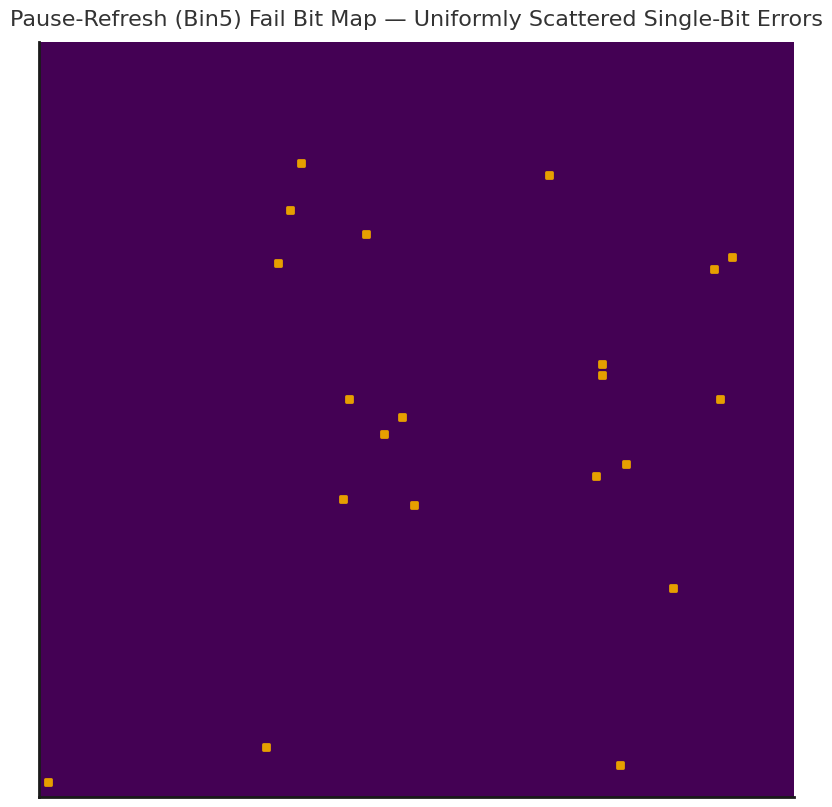
\includegraphics[width=\columnwidth]{fail_bitmap_bin5}
  \caption{Typical fail bit map under pause-refresh test (Bin5).
  Uniformly scattered single-bit errors are observed without edge/line signatures.}
  \label{fig:fail_bitmap}
\end{figure}

\subsection{Hypothesis (Failure Model)}
Directly measurable leakages were normal, suggesting a subtle leakage path. We hypothesized increased leakage at the \textbf{storage-node contact $n^+/p^-$ junction}. After gate etch, a remnant gate oxide on S/D active is repeatedly exposed to resist-stripping \emph{ashing} during multiple LDD steps. Cumulative plasma damage makes the oxide locally porous and can extend damage into the diffusion, creating minute leakage paths. This explains random single-bit distribution without visible structural defects.

% === Storage-node contact n+/p- leakage (TikZ) ===
\begin{figure}[t]
\centering
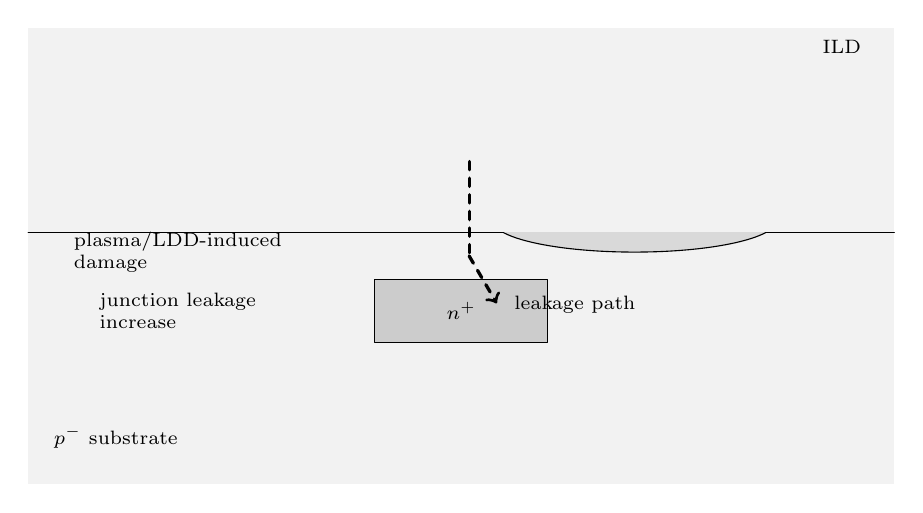
\begin{tikzpicture}[x=1cm,y=1cm,line join=round,line cap=round]
  % ---- styles(グレースケール。数値を変えると濃さ調整)----
  \def\subcol{black!5}   % substrate/ILD
  \def\diffcol{black!20} % n+ diffusion
  \def\gatecol{black!30} % WL
  \def\locoscol{black!15}% LOCOS
  \def\metalcol{black!60}% contact/metal

  % ---- 枠(座標系)----
  \path (-5,-3.2) rectangle (6,2.6);

  % ---- p- substrate & surface ----
  \fill[\subcol] (-5,-3.2) rectangle (6,0);
  \draw (-5,0) -- (6,0);
  \node[anchor=west,font=\scriptsize] at (-4.8,-2.6) {$p^{-}$ substrate};

  % ---- n+ diffusion (storage node diffusion) ----
  \fill[\diffcol] (-0.6,-1.4) rectangle (1.6,-0.6);
  \draw (-0.6,-1.4) rectangle (1.6,-0.6);
  \node[font=\scriptsize] at (0.5,-1.0) {$n^{+}$};

  % ---- Word Line (WL) ----
  \fill[\gatecol] (-2.5,0.10) rectangle (-1.3,0.55);
  \draw (-2.5,0.10) rectangle (-1.3,0.55);
  \node[font=\scriptsize] at (-1.9,0.75) {WL};

  % ---- LOCOS field oxide(鳥のくちばし形状)----
  \fill[\locoscol] (2.7,0.15) ellipse (1.8 and 0.40);
  \draw (2.7,0.15) ellipse (1.8 and 0.40);
  \node[font=\scriptsize] at (4.2,0.75) {LOCOS};

  % ---- Storage-node contact plug → metal → SN ----
  \fill[\metalcol] (0.30,0.00) rectangle (0.90,0.90);        % plug
  \draw (0.30,0.00) rectangle (0.90,0.90);
  \fill[\metalcol] (0.46,0.90) rectangle (0.74,1.15);        % via/metal
  \draw (0.46,0.90) rectangle (0.74,1.15);
  \draw[rounded corners=0.05cm] (-0.10,1.15) rectangle (1.10,1.75); % SN plate
  \node[font=\scriptsize] at (0.50,1.45) {SN};
  \draw[->,>=latex] (1.85,1.60) -- (0.60,0.45);
  \node[anchor=west,font=\scriptsize] at (1.88,1.60) {storage node contact};

  % ---- ILD(上層誘電体)----
  \begin{scope}
    \clip (-5,0) rectangle (6,2.6);
    \fill[\subcol] (-5,0) rectangle (6,2.6);
  \end{scope}
  \node[font=\scriptsize,anchor=east] at (5.7,2.35) {ILD};

  % ---- Leakage path(接触エッジ→接合)----
  \draw[very thick,dashed] (0.60,0.90) -- (0.60,-0.30);
  \draw[very thick,dashed,->] (0.60,-0.30) -- (0.95,-0.90);
  \node[anchor=west,font=\scriptsize] at (1.05,-0.92) {leakage path};

  % ---- 備考(ダメージ起点など)----
  \node[align=left,font=\scriptsize] at (-3.1,-0.25) {plasma/LDD-induced\\damage};
  \node[align=left,font=\scriptsize] at (-3.1,-1.00) {junction leakage\\increase};
\end{tikzpicture}
\caption{Schematic of storage-node contact (n$^+$/p$^-$) leakage.  
Damage near the contact edge increases junction leakage, degrading retention.}
\label{fig:storage_contact}
\end{figure}

\subsection{Countermeasures}
\begin{itemize}
  \item \textbf{Process}: Replace resist stripping in LDD steps from plasma ashing to \textbf{wet stripping (sulfuric-based)} to eliminate plasma damage. 
  \item \textbf{Integration hygiene}: Confirm downstream photo cleanliness and avoid residue risks with the wet strip.
\end{itemize}

\subsection{Effectiveness}
Yield improved from $\sim$65\% to \textbf{$\sim$80\%}. Uniformly scattered single-bit fails decreased markedly. Burn-in and retention/reliability passed; the final recipe was fixed for volume production.

% === Yield-by-lot (step improvement at countermeasure) ===
\begin{figure}[t]
\centering
\pgfplotstableread[col sep=comma]{data/yield_lot.csv}\yieldtbl
\begin{tikzpicture}
\begin{axis}[
  width=\columnwidth, height=0.58\columnwidth,
  xlabel={Lot ID}, ylabel={Yield [\%]},
  ymin=50, ymax=95,
  xmin=0.5, xmax=12.5,
  grid=both,
  xtick=data,
  xticklabels from table={\yieldtbl}{lot},
  xticklabel style={rotate=45, anchor=east},
]
  % データ描画
  \addplot+[mark=*] table[x expr=\coordindex+1, y=yield]{\yieldtbl};

  % 対策境界: lot04とlot05の間
  \draw[dashed] (axis cs:4.5,50) -- (axis cs:4.5,95);
  \node[anchor=west, font=\footnotesize] at (axis cs:4.55,92)
    {Countermeasure};
\end{axis}
\end{tikzpicture}
\caption{Yield step improvement at the countermeasure boundary
between \texttt{lot04} and \texttt{lot05}. Yield jumps from $\sim$62--63\% 
(lot01--lot04) to $\sim$82--84\% (lot05 onward) after changing 
LDD resist stripping from ashing to wet stripping.}
\label{fig:yield}
\end{figure}
